\documentclass[1p]{elsarticle_modified}
%\bibliographystyle{elsarticle-num}

%\usepackage[colorlinks]{hyperref}
%\usepackage{abbrmath_seonhwa} %\Abb, \Ascr, \Acal ,\Abf, \Afrak
\usepackage{amsfonts}
\usepackage{amssymb}
\usepackage{amsmath}
\usepackage{amsthm}
\usepackage{scalefnt}
\usepackage{amsbsy}
\usepackage{kotex}
\usepackage{caption}
\usepackage{subfig}
\usepackage{color}
\usepackage{graphicx}
\usepackage{xcolor} %% white, black, red, green, blue, cyan, magenta, yellow
\usepackage{float}
\usepackage{setspace}
\usepackage{hyperref}

\usepackage{tikz}
\usetikzlibrary{arrows}

\usepackage{multirow}
\usepackage{array} % fixed length table
\usepackage{hhline}

%%%%%%%%%%%%%%%%%%%%%
\makeatletter
\renewcommand*\env@matrix[1][\arraystretch]{%
	\edef\arraystretch{#1}%
	\hskip -\arraycolsep
	\let\@ifnextchar\new@ifnextchar
	\array{*\c@MaxMatrixCols c}}
\makeatother %https://tex.stackexchange.com/questions/14071/how-can-i-increase-the-line-spacing-in-a-matrix
%%%%%%%%%%%%%%%

\usepackage[normalem]{ulem}

\newcommand{\msout}[1]{\ifmmode\text{\sout{\ensuremath{#1}}}\else\sout{#1}\fi}
%SOURCE: \msout is \stkout macro in https://tex.stackexchange.com/questions/20609/strikeout-in-math-mode

\newcommand{\cancel}[1]{
	\ifmmode
	{\color{red}\msout{#1}}
	\else
	{\color{red}\sout{#1}}
	\fi
}

\newcommand{\add}[1]{
	{\color{blue}\uwave{#1}}
}

\newcommand{\replace}[2]{
	\ifmmode
	{\color{red}\msout{#1}}{\color{blue}\uwave{#2}}
	\else
	{\color{red}\sout{#1}}{\color{blue}\uwave{#2}}
	\fi
}

\newcommand{\Sol}{\mathcal{S}} %segment
\newcommand{\D}{D} %diagram
\newcommand{\A}{\mathcal{A}} %arc


%%%%%%%%%%%%%%%%%%%%%%%%%%%%%5 test

\def\sl{\operatorname{\textup{SL}}(2,\Cbb)}
\def\psl{\operatorname{\textup{PSL}}(2,\Cbb)}
\def\quan{\mkern 1mu \triangleright \mkern 1mu}

\theoremstyle{definition}
\newtheorem{thm}{Theorem}[section]
\newtheorem{prop}[thm]{Proposition}
\newtheorem{lem}[thm]{Lemma}
\newtheorem{ques}[thm]{Question}
\newtheorem{cor}[thm]{Corollary}
\newtheorem{defn}[thm]{Definition}
\newtheorem{exam}[thm]{Example}
\newtheorem{rmk}[thm]{Remark}
\newtheorem{alg}[thm]{Algorithm}

\newcommand{\I}{\sqrt{-1}}
\begin{document}

%\begin{frontmatter}
%
%\title{Boundary parabolic representations of knots up to 8 crossings}
%
%%% Group authors per affiliation:
%\author{Yunhi Cho} 
%\address{Department of Mathematics, University of Seoul, Seoul, Korea}
%\ead{yhcho@uos.ac.kr}
%
%
%\author{Seonhwa Kim} %\fnref{s_kim}}
%\address{Center for Geometry and Physics, Institute for Basic Science, Pohang, 37673, Korea}
%\ead{ryeona17@ibs.re.kr}
%
%\author{Hyuk Kim}
%\address{Department of Mathematical Sciences, Seoul National University, Seoul 08826, Korea}
%\ead{hyukkim@snu.ac.kr}
%
%\author{Seokbeom Yoon}
%\address{Department of Mathematical Sciences, Seoul National University, Seoul, 08826,  Korea}
%\ead{sbyoon15@snu.ac.kr}
%
%\begin{abstract}
%We find all boundary parabolic representation of knots up to 8 crossings.
%
%\end{abstract}
%\begin{keyword}
%    \MSC[2010] 57M25 
%\end{keyword}
%
%\end{frontmatter}

%\linenumbers
%\tableofcontents
%
\newcommand\colored[1]{\textcolor{white}{\rule[-0.35ex]{0.8em}{1.4ex}}\kern-0.8em\color{red} #1}%
%\newcommand\colored[1]{\textcolor{white}{ #1}\kern-2.17ex	\textcolor{white}{ #1}\kern-1.81ex	\textcolor{white}{ #1}\kern-2.15ex\color{red}#1	}

{\Large $\underline{11a_{2}~(K11a_{2})}$}

\setlength{\tabcolsep}{10pt}
\renewcommand{\arraystretch}{1.6}
\vspace{1cm}\begin{tabular}{m{100pt}>{\centering\arraybackslash}m{274pt}}
\multirow{5}{120pt}{
	\centering
	\includegraphics[width=112pt]{../../../GIT/diagram.site/Diagrams/png/251_11a_2.png}\\
\ \ \ A knot diagram\footnotemark}&
\allowdisplaybreaks
\textbf{Linearized knot diagam} \\
\cline{2-2}
 &
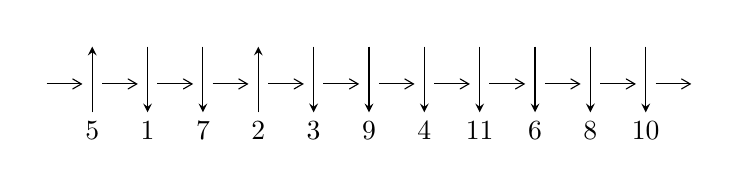
\begin{tikzpicture}[x=20pt, y=17pt]
	% nodes
	\node (C0) at (0, 0) {};
	\node (C1) at (1, 0) {};
	\node (C1U) at (1, +1) {};
	\node (C1D) at (1, -1) {5};

	\node (C2) at (2, 0) {};
	\node (C2U) at (2, +1) {};
	\node (C2D) at (2, -1) {1};

	\node (C3) at (3, 0) {};
	\node (C3U) at (3, +1) {};
	\node (C3D) at (3, -1) {7};

	\node (C4) at (4, 0) {};
	\node (C4U) at (4, +1) {};
	\node (C4D) at (4, -1) {2};

	\node (C5) at (5, 0) {};
	\node (C5U) at (5, +1) {};
	\node (C5D) at (5, -1) {3};

	\node (C6) at (6, 0) {};
	\node (C6U) at (6, +1) {};
	\node (C6D) at (6, -1) {9};

	\node (C7) at (7, 0) {};
	\node (C7U) at (7, +1) {};
	\node (C7D) at (7, -1) {4};

	\node (C8) at (8, 0) {};
	\node (C8U) at (8, +1) {};
	\node (C8D) at (8, -1) {11};

	\node (C9) at (9, 0) {};
	\node (C9U) at (9, +1) {};
	\node (C9D) at (9, -1) {6};

	\node (C10) at (10, 0) {};
	\node (C10U) at (10, +1) {};
	\node (C10D) at (10, -1) {8};

	\node (C11) at (11, 0) {};
	\node (C11U) at (11, +1) {};
	\node (C11D) at (11, -1) {10};
	\node (C12) at (12, 0) {};

	% arrows
	\draw[->,>={angle 60}]
	(C0) edge (C1) (C1) edge (C2) (C2) edge (C3) (C3) edge (C4) (C4) edge (C5) (C5) edge (C6) (C6) edge (C7) (C7) edge (C8) (C8) edge (C9) (C9) edge (C10) (C10) edge (C11) (C11) edge (C12) ;	\draw[->,>=stealth]
	(C1D) edge (C1U) (C2U) edge (C2D) (C3U) edge (C3D) (C4D) edge (C4U) (C5U) edge (C5D) (C6U) edge (C6D) (C7U) edge (C7D) (C8U) edge (C8D) (C9U) edge (C9D) (C10U) edge (C10D) (C11U) edge (C11D) ;
	\end{tikzpicture} \\
\hhline{~~} \\& 
\textbf{Solving Sequence} \\ \cline{2-2} 
 &
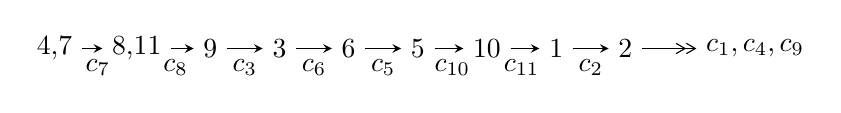
\begin{tikzpicture}[x=25pt, y=7pt]
	% node
	\node (A0) at (-1/8, 0) {4,7};
	\node (A1) at (17/16, 0) {8,11};
	\node (A2) at (17/8, 0) {9};
	\node (A3) at (25/8, 0) {3};
	\node (A4) at (33/8, 0) {6};
	\node (A5) at (41/8, 0) {5};
	\node (A6) at (49/8, 0) {10};
	\node (A7) at (57/8, 0) {1};
	\node (A8) at (65/8, 0) {2};
	\node (C1) at (1/2, -1) {$c_{7}$};
	\node (C2) at (13/8, -1) {$c_{8}$};
	\node (C3) at (21/8, -1) {$c_{3}$};
	\node (C4) at (29/8, -1) {$c_{6}$};
	\node (C5) at (37/8, -1) {$c_{5}$};
	\node (C6) at (45/8, -1) {$c_{10}$};
	\node (C7) at (53/8, -1) {$c_{11}$};
	\node (C8) at (61/8, -1) {$c_{2}$};
	\node (A9) at (10, 0) {$c_{1},c_{4},c_{9}$};

	% edge
	\draw[->,>=stealth]	
	(A0) edge (A1) (A1) edge (A2) (A2) edge (A3) (A3) edge (A4) (A4) edge (A5) (A5) edge (A6) (A6) edge (A7) (A7) edge (A8) ;
	\draw[->>,>={angle 60}]	
	(A8) edge (A9);
\end{tikzpicture} \\ 

\end{tabular} \\

\footnotetext{
The image of knot diagram is generated by the software ``\textbf{Draw programme}" developed by Andrew Bartholomew(\url{http://www.layer8.co.uk/maths/draw/index.htm\#Running-draw}), where we modified some parts for our purpose(\url{https://github.com/CATsTAILs/LinksPainter}).
}\phantom \\ \newline 
\centering \textbf{Ideals for irreducible components\footnotemark of $X_{\text{par}}$} 
 
\begin{align*}
I^u_{1}&=\langle 
-5.43741\times10^{171} u^{78}-5.11274\times10^{171} u^{77}+\cdots+1.98334\times10^{172} b-2.82335\times10^{173},\\
\phantom{I^u_{1}}&\phantom{= \langle  }-1.22224\times10^{171} u^{78}+1.44341\times10^{172} u^{77}+\cdots+1.58667\times10^{173} a+1.86038\times10^{174},\\
\phantom{I^u_{1}}&\phantom{= \langle  }u^{79}+2 u^{78}+\cdots+224 u+64\rangle \\
I^u_{2}&=\langle 
u^2+b,\;u^4-2 u^3- u^2+a+3 u+1,\;u^5- u^4-2 u^3+u^2+u+1\rangle \\
\\
I^v_{1}&=\langle 
a,\;-18 v^5-63 v^4-193 v^3-63 v^2+55 b+27 v+12,\;v^6+2 v^5+7 v^4-8 v^3+7 v^2-3 v+1\rangle \\
\end{align*}
\raggedright * 3 irreducible components of $\dim_{\mathbb{C}}=0$, with total 90 representations.\\
\footnotetext{All coefficients of polynomials are rational numbers. But the coefficients are sometimes approximated in decimal forms when there is not enough margin.}
\newpage
\renewcommand{\arraystretch}{1}
\centering \section*{I. $I^u_{1}= \langle -5.44\times10^{171} u^{78}-5.11\times10^{171} u^{77}+\cdots+1.98\times10^{172} b-2.82\times10^{173},\;-1.22\times10^{171} u^{78}+1.44\times10^{172} u^{77}+\cdots+1.59\times10^{173} a+1.86\times10^{174},\;u^{79}+2 u^{78}+\cdots+224 u+64 \rangle$}
\flushleft \textbf{(i) Arc colorings}\\
\begin{tabular}{m{7pt} m{180pt} m{7pt} m{180pt} }
\flushright $a_{4}=$&$\begin{pmatrix}0\\u\end{pmatrix}$ \\
\flushright $a_{7}=$&$\begin{pmatrix}1\\0\end{pmatrix}$ \\
\flushright $a_{8}=$&$\begin{pmatrix}1\\u^2\end{pmatrix}$ \\
\flushright $a_{11}=$&$\begin{pmatrix}0.00770315 u^{78}-0.0909705 u^{77}+\cdots-27.2773 u-11.7250\\0.274154 u^{78}+0.257784 u^{77}+\cdots+36.6907 u+14.2353\end{pmatrix}$ \\
\flushright $a_{9}=$&$\begin{pmatrix}0.0515299 u^{78}-0.0134218 u^{77}+\cdots-14.2684 u-3.89351\\-0.204276 u^{78}-0.212923 u^{77}+\cdots-35.5855 u-11.5905\end{pmatrix}$ \\
\flushright $a_{3}=$&$\begin{pmatrix}u\\u\end{pmatrix}$ \\
\flushright $a_{6}=$&$\begin{pmatrix}-0.0432551 u^{78}-0.0953382 u^{77}+\cdots-17.7659 u-9.19854\\0.0600517 u^{78}+0.0392781 u^{77}+\cdots+5.74611 u-3.52633\end{pmatrix}$ \\
\flushright $a_{5}=$&$\begin{pmatrix}-0.0400019 u^{78}-0.0348387 u^{77}+\cdots-8.25015 u-4.59071\\0.0633049 u^{78}+0.0997776 u^{77}+\cdots+15.2619 u+1.08150\end{pmatrix}$ \\
\flushright $a_{10}=$&$\begin{pmatrix}0.102479 u^{78}-0.00813482 u^{77}+\cdots-13.9221 u-4.29785\\0.401016 u^{78}+0.368694 u^{77}+\cdots+54.5295 u+21.0651\end{pmatrix}$ \\
\flushright $a_{1}=$&$\begin{pmatrix}-0.103307 u^{78}-0.134616 u^{77}+\cdots-23.5120 u-5.67221\\-0.0633049 u^{78}-0.0997776 u^{77}+\cdots-15.2619 u-1.08150\end{pmatrix}$ \\
\flushright $a_{2}=$&$\begin{pmatrix}0.140138 u^{78}+0.241968 u^{77}+\cdots+33.5462 u+15.5291\\0.278386 u^{78}+0.429982 u^{77}+\cdots+64.6729 u+27.3218\end{pmatrix}$\\ \flushright $a_{2}=$&$\begin{pmatrix}0.140138 u^{78}+0.241968 u^{77}+\cdots+33.5462 u+15.5291\\0.278386 u^{78}+0.429982 u^{77}+\cdots+64.6729 u+27.3218\end{pmatrix}$\\&\end{tabular}
\flushleft \textbf{(ii) Obstruction class $= -1$}\\~\\
\flushleft \textbf{(iii) Cusp Shapes $= -0.0683647 u^{78}+0.114454 u^{77}+\cdots-17.3139 u-1.86024$}\\~\\
\newpage\renewcommand{\arraystretch}{1}
\flushleft \textbf{(iv) u-Polynomials at the component}\newline \\
\begin{tabular}{m{50pt}|m{274pt}}
Crossings & \hspace{64pt}u-Polynomials at each crossing \\
\hline $$\begin{aligned}c_{1},c_{4}\end{aligned}$$&$\begin{aligned}
&u^{79}+5 u^{78}+\cdots+12 u+1
\end{aligned}$\\
\hline $$\begin{aligned}c_{2}\end{aligned}$$&$\begin{aligned}
&u^{79}+39 u^{78}+\cdots+42 u-1
\end{aligned}$\\
\hline $$\begin{aligned}c_{3},c_{7}\end{aligned}$$&$\begin{aligned}
&u^{79}+2 u^{78}+\cdots+224 u+64
\end{aligned}$\\
\hline $$\begin{aligned}c_{5}\end{aligned}$$&$\begin{aligned}
&u^{79}-5 u^{78}+\cdots+14176 u+3137
\end{aligned}$\\
\hline $$\begin{aligned}c_{6},c_{9}\end{aligned}$$&$\begin{aligned}
&u^{79}-3 u^{78}+\cdots-192 u+32
\end{aligned}$\\
\hline $$\begin{aligned}c_{8},c_{10}\end{aligned}$$&$\begin{aligned}
&u^{79}-8 u^{78}+\cdots-5 u+1
\end{aligned}$\\
\hline $$\begin{aligned}c_{11}\end{aligned}$$&$\begin{aligned}
&u^{79}+38 u^{78}+\cdots-137 u+1
\end{aligned}$\\
\hline
\end{tabular}\\~\\
\newpage\renewcommand{\arraystretch}{1}
\flushleft \textbf{(v) Riley Polynomials at the component}\newline \\
\begin{tabular}{m{50pt}|m{274pt}}
Crossings & \hspace{64pt}Riley Polynomials at each crossing \\
\hline $$\begin{aligned}c_{1},c_{4}\end{aligned}$$&$\begin{aligned}
&y^{79}+39 y^{78}+\cdots+42 y-1
\end{aligned}$\\
\hline $$\begin{aligned}c_{2}\end{aligned}$$&$\begin{aligned}
&y^{79}+7 y^{78}+\cdots+2238 y-1
\end{aligned}$\\
\hline $$\begin{aligned}c_{3},c_{7}\end{aligned}$$&$\begin{aligned}
&y^{79}-40 y^{78}+\cdots+91136 y-4096
\end{aligned}$\\
\hline $$\begin{aligned}c_{5}\end{aligned}$$&$\begin{aligned}
&y^{79}-25 y^{78}+\cdots+636907866 y-9840769
\end{aligned}$\\
\hline $$\begin{aligned}c_{6},c_{9}\end{aligned}$$&$\begin{aligned}
&y^{79}+39 y^{78}+\cdots-15872 y-1024
\end{aligned}$\\
\hline $$\begin{aligned}c_{8},c_{10}\end{aligned}$$&$\begin{aligned}
&y^{79}-38 y^{78}+\cdots-137 y-1
\end{aligned}$\\
\hline $$\begin{aligned}c_{11}\end{aligned}$$&$\begin{aligned}
&y^{79}+14 y^{78}+\cdots+11687 y-1
\end{aligned}$\\
\hline
\end{tabular}\\~\\
\newpage\flushleft \textbf{(vi) Complex Volumes and Cusp Shapes}
$$\begin{array}{c|c|c}  
\text{Solutions to }I^u_{1}& \I (\text{vol} + \sqrt{-1}CS) & \text{Cusp shape}\\
 \hline 
\begin{aligned}
u &= -0.853592 + 0.508882 I \\
a &= -0.055782 + 1.086980 I \\
b &= \phantom{-}0.385053 - 0.112918 I\end{aligned}
 & \phantom{-}2.66697 - 2.36282 I & -4.65001 + 1.65972 I \\ \hline\begin{aligned}
u &= -0.853592 - 0.508882 I \\
a &= -0.055782 - 1.086980 I \\
b &= \phantom{-}0.385053 + 0.112918 I\end{aligned}
 & \phantom{-}2.66697 + 2.36282 I & -4.65001 - 1.65972 I \\ \hline\begin{aligned}
u &= -0.440363 + 0.912546 I \\
a &= \phantom{-}0.724174 + 0.449379 I \\
b &= -0.699520 - 0.426408 I\end{aligned}
 & -0.27585 + 2.15811 I & -7.00000 - 4.29711 I \\ \hline\begin{aligned}
u &= -0.440363 - 0.912546 I \\
a &= \phantom{-}0.724174 - 0.449379 I \\
b &= -0.699520 + 0.426408 I\end{aligned}
 & -0.27585 - 2.15811 I & -7.00000 + 4.29711 I \\ \hline\begin{aligned}
u &= \phantom{-}0.320495 + 0.912395 I \\
a &= \phantom{-}0.249632 - 0.939746 I \\
b &= \phantom{-}1.37567 + 0.42738 I\end{aligned}
 & -2.34704 + 4.31468 I & -10.21762 - 4.57210 I \\ \hline\begin{aligned}
u &= \phantom{-}0.320495 - 0.912395 I \\
a &= \phantom{-}0.249632 + 0.939746 I \\
b &= \phantom{-}1.37567 - 0.42738 I\end{aligned}
 & -2.34704 - 4.31468 I & -10.21762 + 4.57210 I \\ \hline\begin{aligned}
u &= \phantom{-}0.567410 + 0.878865 I \\
a &= \phantom{-}0.595821 - 0.532012 I \\
b &= -0.237797 + 0.089887 I\end{aligned}
 & \phantom{-}3.87103 - 0.09665 I & \phantom{-0.000000 } 0 \\ \hline\begin{aligned}
u &= \phantom{-}0.567410 - 0.878865 I \\
a &= \phantom{-}0.595821 + 0.532012 I \\
b &= -0.237797 - 0.089887 I\end{aligned}
 & \phantom{-}3.87103 + 0.09665 I & \phantom{-0.000000 } 0 \\ \hline\begin{aligned}
u &= -0.890520 + 0.328701 I \\
a &= \phantom{-}0.424564 + 0.261362 I \\
b &= \phantom{-}0.946519 + 0.465471 I\end{aligned}
 & -1.024930 + 0.378054 I & -6.69847 + 0.35322 I \\ \hline\begin{aligned}
u &= -0.890520 - 0.328701 I \\
a &= \phantom{-}0.424564 - 0.261362 I \\
b &= \phantom{-}0.946519 - 0.465471 I\end{aligned}
 & -1.024930 - 0.378054 I & -6.69847 - 0.35322 I\\
 \hline 
 \end{array}$$\newpage$$\begin{array}{c|c|c}  
\text{Solutions to }I^u_{1}& \I (\text{vol} + \sqrt{-1}CS) & \text{Cusp shape}\\
 \hline 
\begin{aligned}
u &= \phantom{-}0.913716 + 0.570561 I \\
a &= -0.226843 - 0.736350 I \\
b &= \phantom{-}0.189637 + 0.143627 I\end{aligned}
 & \phantom{-}3.68282 - 2.87436 I & \phantom{-0.000000 } 0 \\ \hline\begin{aligned}
u &= \phantom{-}0.913716 - 0.570561 I \\
a &= -0.226843 + 0.736350 I \\
b &= \phantom{-}0.189637 - 0.143627 I\end{aligned}
 & \phantom{-}3.68282 + 2.87436 I & \phantom{-0.000000 } 0 \\ \hline\begin{aligned}
u &= -1.045420 + 0.303052 I \\
a &= \phantom{-}2.58858 + 0.40116 I \\
b &= \phantom{-}1.81492 - 0.66339 I\end{aligned}
 & \phantom{-}1.18747 + 2.48169 I & \phantom{-0.000000 } 0 \\ \hline\begin{aligned}
u &= -1.045420 - 0.303052 I \\
a &= \phantom{-}2.58858 - 0.40116 I \\
b &= \phantom{-}1.81492 + 0.66339 I\end{aligned}
 & \phantom{-}1.18747 - 2.48169 I & \phantom{-0.000000 } 0 \\ \hline\begin{aligned}
u &= -0.809973 + 0.391729 I \\
a &= \phantom{-}0.515617 + 0.419812 I \\
b &= -0.258885 + 0.774414 I\end{aligned}
 & \phantom{-}2.91495 + 6.10945 I & -7.82272 - 8.97445 I \\ \hline\begin{aligned}
u &= -0.809973 - 0.391729 I \\
a &= \phantom{-}0.515617 - 0.419812 I \\
b &= -0.258885 - 0.774414 I\end{aligned}
 & \phantom{-}2.91495 - 6.10945 I & -7.82272 + 8.97445 I \\ \hline\begin{aligned}
u &= \phantom{-}0.404716 + 1.023830 I \\
a &= \phantom{-}0.584705 + 0.288653 I \\
b &= -1.81023 + 0.83355 I\end{aligned}
 & \phantom{-}2.22736 + 5.03014 I & \phantom{-0.000000 } 0 \\ \hline\begin{aligned}
u &= \phantom{-}0.404716 - 1.023830 I \\
a &= \phantom{-}0.584705 - 0.288653 I \\
b &= -1.81023 - 0.83355 I\end{aligned}
 & \phantom{-}2.22736 - 5.03014 I & \phantom{-0.000000 } 0 \\ \hline\begin{aligned}
u &= \phantom{-}0.653865 + 0.591272 I \\
a &= \phantom{-}0.546637 - 0.447428 I \\
b &= -0.313726 - 0.436492 I\end{aligned}
 & \phantom{-}4.46313 - 1.71758 I & -1.99294 + 3.91162 I \\ \hline\begin{aligned}
u &= \phantom{-}0.653865 - 0.591272 I \\
a &= \phantom{-}0.546637 + 0.447428 I \\
b &= -0.313726 + 0.436492 I\end{aligned}
 & \phantom{-}4.46313 + 1.71758 I & -1.99294 - 3.91162 I\\
 \hline 
 \end{array}$$\newpage$$\begin{array}{c|c|c}  
\text{Solutions to }I^u_{1}& \I (\text{vol} + \sqrt{-1}CS) & \text{Cusp shape}\\
 \hline 
\begin{aligned}
u &= -0.543636 + 0.978739 I \\
a &= \phantom{-}0.595952 + 0.594331 I \\
b &= -0.143500 - 0.270257 I\end{aligned}
 & \phantom{-}1.84084 - 4.64712 I & \phantom{-0.000000 } 0 \\ \hline\begin{aligned}
u &= -0.543636 - 0.978739 I \\
a &= \phantom{-}0.595952 - 0.594331 I \\
b &= -0.143500 + 0.270257 I\end{aligned}
 & \phantom{-}1.84084 + 4.64712 I & \phantom{-0.000000 } 0 \\ \hline\begin{aligned}
u &= \phantom{-}1.136340 + 0.085967 I \\
a &= \phantom{-}0.279099 - 0.088232 I \\
b &= \phantom{-}0.651828 - 0.756122 I\end{aligned}
 & -4.51217 + 2.77386 I & \phantom{-0.000000 } 0 \\ \hline\begin{aligned}
u &= \phantom{-}1.136340 - 0.085967 I \\
a &= \phantom{-}0.279099 + 0.088232 I \\
b &= \phantom{-}0.651828 + 0.756122 I\end{aligned}
 & -4.51217 - 2.77386 I & \phantom{-0.000000 } 0 \\ \hline\begin{aligned}
u &= \phantom{-}1.067750 + 0.420888 I \\
a &= -1.87786 + 0.34577 I \\
b &= -0.83129 - 1.54411 I\end{aligned}
 & -3.40761 - 2.20375 I & \phantom{-0.000000 } 0 \\ \hline\begin{aligned}
u &= \phantom{-}1.067750 - 0.420888 I \\
a &= -1.87786 - 0.34577 I \\
b &= -0.83129 + 1.54411 I\end{aligned}
 & -3.40761 + 2.20375 I & \phantom{-0.000000 } 0 \\ \hline\begin{aligned}
u &= -0.125465 + 0.835214 I \\
a &= -0.10435 - 1.59020 I \\
b &= \phantom{-}0.862564 + 0.893320 I\end{aligned}
 & -2.81805 - 2.16506 I & -9.87540 + 5.61737 I \\ \hline\begin{aligned}
u &= -0.125465 - 0.835214 I \\
a &= -0.10435 + 1.59020 I \\
b &= \phantom{-}0.862564 - 0.893320 I\end{aligned}
 & -2.81805 + 2.16506 I & -9.87540 - 5.61737 I \\ \hline\begin{aligned}
u &= \phantom{-}1.074320 + 0.446434 I \\
a &= \phantom{-}2.33317 - 0.78177 I \\
b &= \phantom{-}1.90096 + 0.89090 I\end{aligned}
 & \phantom{-}1.85989 - 8.01595 I & \phantom{-0.000000 } 0 \\ \hline\begin{aligned}
u &= \phantom{-}1.074320 - 0.446434 I \\
a &= \phantom{-}2.33317 + 0.78177 I \\
b &= \phantom{-}1.90096 - 0.89090 I\end{aligned}
 & \phantom{-}1.85989 + 8.01595 I & \phantom{-0.000000 } 0\\
 \hline 
 \end{array}$$\newpage$$\begin{array}{c|c|c}  
\text{Solutions to }I^u_{1}& \I (\text{vol} + \sqrt{-1}CS) & \text{Cusp shape}\\
 \hline 
\begin{aligned}
u &= -0.725121 + 0.392006 I \\
a &= -1.90522 - 2.47065 I \\
b &= -1.210690 - 0.210584 I\end{aligned}
 & -0.64046 + 2.98061 I & -8.98738 - 7.04047 I \\ \hline\begin{aligned}
u &= -0.725121 - 0.392006 I \\
a &= -1.90522 + 2.47065 I \\
b &= -1.210690 + 0.210584 I\end{aligned}
 & -0.64046 - 2.98061 I & -8.98738 + 7.04047 I \\ \hline\begin{aligned}
u &= \phantom{-}1.104970 + 0.414939 I \\
a &= \phantom{-}0.283959 - 0.271043 I \\
b &= \phantom{-}1.069610 - 0.727261 I\end{aligned}
 & -3.45530 - 4.80167 I & \phantom{-0.000000 } 0 \\ \hline\begin{aligned}
u &= \phantom{-}1.104970 - 0.414939 I \\
a &= \phantom{-}0.283959 + 0.271043 I \\
b &= \phantom{-}1.069610 + 0.727261 I\end{aligned}
 & -3.45530 + 4.80167 I & \phantom{-0.000000 } 0 \\ \hline\begin{aligned}
u &= -0.170048 + 1.184850 I \\
a &= \phantom{-}0.627452 - 0.278541 I \\
b &= -1.99843 - 0.37107 I\end{aligned}
 & -1.69051 - 1.86503 I & \phantom{-0.000000 } 0 \\ \hline\begin{aligned}
u &= -0.170048 - 1.184850 I \\
a &= \phantom{-}0.627452 + 0.278541 I \\
b &= -1.99843 + 0.37107 I\end{aligned}
 & -1.69051 + 1.86503 I & \phantom{-0.000000 } 0 \\ \hline\begin{aligned}
u &= -0.441408 + 0.647966 I \\
a &= \phantom{-}0.543640 + 0.757595 I \\
b &= \phantom{-}1.160190 - 0.111260 I\end{aligned}
 & -0.501227 - 0.231040 I & -6.51195 + 0.36059 I \\ \hline\begin{aligned}
u &= -0.441408 - 0.647966 I \\
a &= \phantom{-}0.543640 - 0.757595 I \\
b &= \phantom{-}1.160190 + 0.111260 I\end{aligned}
 & -0.501227 + 0.231040 I & -6.51195 - 0.36059 I \\ \hline\begin{aligned}
u &= -1.101140 + 0.524739 I \\
a &= -1.31740 - 1.35522 I \\
b &= -1.76932 - 0.29287 I\end{aligned}
 & -2.56199 + 4.84000 I & \phantom{-0.000000 } 0 \\ \hline\begin{aligned}
u &= -1.101140 - 0.524739 I \\
a &= -1.31740 + 1.35522 I \\
b &= -1.76932 + 0.29287 I\end{aligned}
 & -2.56199 - 4.84000 I & \phantom{-0.000000 } 0\\
 \hline 
 \end{array}$$\newpage$$\begin{array}{c|c|c}  
\text{Solutions to }I^u_{1}& \I (\text{vol} + \sqrt{-1}CS) & \text{Cusp shape}\\
 \hline 
\begin{aligned}
u &= -0.743273 + 0.192362 I \\
a &= \phantom{-}0.523153 - 0.357954 I \\
b &= -0.778082 - 1.165960 I\end{aligned}
 & \phantom{-}2.43852 - 0.18703 I & -11.37446 - 3.74898 I \\ \hline\begin{aligned}
u &= -0.743273 - 0.192362 I \\
a &= \phantom{-}0.523153 + 0.357954 I \\
b &= -0.778082 + 1.165960 I\end{aligned}
 & \phantom{-}2.43852 + 0.18703 I & -11.37446 + 3.74898 I \\ \hline\begin{aligned}
u &= -1.214390 + 0.237157 I \\
a &= -1.81606 + 0.08423 I \\
b &= -1.24455 + 1.45461 I\end{aligned}
 & -7.51790 - 0.99407 I & \phantom{-0.000000 } 0 \\ \hline\begin{aligned}
u &= -1.214390 - 0.237157 I \\
a &= -1.81606 - 0.08423 I \\
b &= -1.24455 - 1.45461 I\end{aligned}
 & -7.51790 + 0.99407 I & \phantom{-0.000000 } 0 \\ \hline\begin{aligned}
u &= -1.148700 + 0.510777 I \\
a &= -0.065466 + 0.259649 I \\
b &= \phantom{-}0.003288 - 0.501341 I\end{aligned}
 & -2.69356 + 2.85282 I & \phantom{-0.000000 } 0 \\ \hline\begin{aligned}
u &= -1.148700 - 0.510777 I \\
a &= -0.065466 - 0.259649 I \\
b &= \phantom{-}0.003288 + 0.501341 I\end{aligned}
 & -2.69356 - 2.85282 I & \phantom{-0.000000 } 0 \\ \hline\begin{aligned}
u &= \phantom{-}1.208390 + 0.353192 I \\
a &= -1.51238 + 1.05060 I \\
b &= -1.79615 + 0.61356 I\end{aligned}
 & -7.01716 - 1.79468 I & \phantom{-0.000000 } 0 \\ \hline\begin{aligned}
u &= \phantom{-}1.208390 - 0.353192 I \\
a &= -1.51238 - 1.05060 I \\
b &= -1.79615 - 0.61356 I\end{aligned}
 & -7.01716 + 1.79468 I & \phantom{-0.000000 } 0 \\ \hline\begin{aligned}
u &= -0.484551 + 1.171980 I \\
a &= \phantom{-}0.580134 - 0.265852 I \\
b &= -2.07365 - 0.94054 I\end{aligned}
 & -0.30685 - 9.73004 I & \phantom{-0.000000 } 0 \\ \hline\begin{aligned}
u &= -0.484551 - 1.171980 I \\
a &= \phantom{-}0.580134 + 0.265852 I \\
b &= -2.07365 + 0.94054 I\end{aligned}
 & -0.30685 + 9.73004 I & \phantom{-0.000000 } 0\\
 \hline 
 \end{array}$$\newpage$$\begin{array}{c|c|c}  
\text{Solutions to }I^u_{1}& \I (\text{vol} + \sqrt{-1}CS) & \text{Cusp shape}\\
 \hline 
\begin{aligned}
u &= \phantom{-}0.516322 + 0.514627 I \\
a &= \phantom{-}0.550028 + 0.336051 I \\
b &= -1.15619 + 1.03408 I\end{aligned}
 & \phantom{-}3.64506 + 4.10175 I & -3.50068 + 0.16550 I \\ \hline\begin{aligned}
u &= \phantom{-}0.516322 - 0.514627 I \\
a &= \phantom{-}0.550028 - 0.336051 I \\
b &= -1.15619 - 1.03408 I\end{aligned}
 & \phantom{-}3.64506 - 4.10175 I & -3.50068 - 0.16550 I \\ \hline\begin{aligned}
u &= \phantom{-}1.098620 + 0.654049 I \\
a &= -0.259825 - 0.296004 I \\
b &= -0.127365 + 0.305299 I\end{aligned}
 & \phantom{-}2.17633 - 5.60365 I & \phantom{-0.000000 } 0 \\ \hline\begin{aligned}
u &= \phantom{-}1.098620 - 0.654049 I \\
a &= -0.259825 + 0.296004 I \\
b &= -0.127365 - 0.305299 I\end{aligned}
 & \phantom{-}2.17633 + 5.60365 I & \phantom{-0.000000 } 0 \\ \hline\begin{aligned}
u &= -1.187720 + 0.505810 I \\
a &= -1.63010 - 0.30290 I \\
b &= -0.89789 + 1.80532 I\end{aligned}
 & -5.97333 + 6.98094 I & \phantom{-0.000000 } 0 \\ \hline\begin{aligned}
u &= -1.187720 - 0.505810 I \\
a &= -1.63010 + 0.30290 I \\
b &= -0.89789 - 1.80532 I\end{aligned}
 & -5.97333 - 6.98094 I & \phantom{-0.000000 } 0 \\ \hline\begin{aligned}
u &= \phantom{-}1.192530 + 0.590288 I \\
a &= -1.17833 + 1.23110 I \\
b &= -1.94360 + 0.25893 I\end{aligned}
 & -5.05086 - 9.82294 I & \phantom{-0.000000 } 0 \\ \hline\begin{aligned}
u &= \phantom{-}1.192530 - 0.590288 I \\
a &= -1.17833 - 1.23110 I \\
b &= -1.94360 - 0.25893 I\end{aligned}
 & -5.05086 + 9.82294 I & \phantom{-0.000000 } 0 \\ \hline\begin{aligned}
u &= \phantom{-}0.453727 + 0.479176 I \\
a &= -1.88077 + 2.61755 I \\
b &= \phantom{-}0.031595 - 0.872947 I\end{aligned}
 & -1.61075 - 1.37550 I & \phantom{-}1.06828 + 3.88421 I \\ \hline\begin{aligned}
u &= \phantom{-}0.453727 - 0.479176 I \\
a &= -1.88077 - 2.61755 I \\
b &= \phantom{-}0.031595 + 0.872947 I\end{aligned}
 & -1.61075 + 1.37550 I & \phantom{-}1.06828 - 3.88421 I\\
 \hline 
 \end{array}$$\newpage$$\begin{array}{c|c|c}  
\text{Solutions to }I^u_{1}& \I (\text{vol} + \sqrt{-1}CS) & \text{Cusp shape}\\
 \hline 
\begin{aligned}
u &= -1.160930 + 0.693518 I \\
a &= -0.270422 + 0.204754 I \\
b &= -0.238385 - 0.350820 I\end{aligned}
 & -0.15331 + 10.78920 I & \phantom{-0.000000 } 0 \\ \hline\begin{aligned}
u &= -1.160930 - 0.693518 I \\
a &= -0.270422 - 0.204754 I \\
b &= -0.238385 + 0.350820 I\end{aligned}
 & -0.15331 - 10.78920 I & \phantom{-0.000000 } 0 \\ \hline\begin{aligned}
u &= \phantom{-}1.218660 + 0.679170 I \\
a &= \phantom{-}1.73476 - 0.94207 I \\
b &= \phantom{-}2.16330 + 1.28301 I\end{aligned}
 & -0.31155 - 11.22020 I & \phantom{-0.000000 } 0 \\ \hline\begin{aligned}
u &= \phantom{-}1.218660 - 0.679170 I \\
a &= \phantom{-}1.73476 + 0.94207 I \\
b &= \phantom{-}2.16330 - 1.28301 I\end{aligned}
 & -0.31155 + 11.22020 I & \phantom{-0.000000 } 0 \\ \hline\begin{aligned}
u &= -1.387240 + 0.184587 I \\
a &= \phantom{-}1.57267 + 0.32546 I \\
b &= \phantom{-}2.17449 - 0.52478 I\end{aligned}
 & -4.07832 - 1.19726 I & \phantom{-0.000000 } 0 \\ \hline\begin{aligned}
u &= -1.387240 - 0.184587 I \\
a &= \phantom{-}1.57267 - 0.32546 I \\
b &= \phantom{-}2.17449 + 0.52478 I\end{aligned}
 & -4.07832 + 1.19726 I & \phantom{-0.000000 } 0 \\ \hline\begin{aligned}
u &= -0.195618 + 0.552066 I \\
a &= \phantom{-}1.178600 + 0.372591 I \\
b &= -0.235368 - 0.239587 I\end{aligned}
 & -0.36323 + 1.66196 I & -2.66065 - 3.49504 I \\ \hline\begin{aligned}
u &= -0.195618 - 0.552066 I \\
a &= \phantom{-}1.178600 - 0.372591 I \\
b &= -0.235368 + 0.239587 I\end{aligned}
 & -0.36323 - 1.66196 I & -2.66065 + 3.49504 I \\ \hline\begin{aligned}
u &= -1.32645 + 0.58089 I \\
a &= \phantom{-}1.73200 + 0.69897 I \\
b &= \phantom{-}2.36240 - 1.10492 I\end{aligned}
 & -5.48277 + 8.06356 I & \phantom{-0.000000 } 0 \\ \hline\begin{aligned}
u &= -1.32645 - 0.58089 I \\
a &= \phantom{-}1.73200 - 0.69897 I \\
b &= \phantom{-}2.36240 + 1.10492 I\end{aligned}
 & -5.48277 - 8.06356 I & \phantom{-0.000000 } 0\\
 \hline 
 \end{array}$$\newpage$$\begin{array}{c|c|c}  
\text{Solutions to }I^u_{1}& \I (\text{vol} + \sqrt{-1}CS) & \text{Cusp shape}\\
 \hline 
\begin{aligned}
u &= -1.25392 + 0.74743 I \\
a &= \phantom{-}1.60645 + 0.95537 I \\
b &= \phantom{-}2.22097 - 1.40824 I\end{aligned}
 & -2.7949 + 16.5881 I & \phantom{-0.000000 } 0 \\ \hline\begin{aligned}
u &= -1.25392 - 0.74743 I \\
a &= \phantom{-}1.60645 - 0.95537 I \\
b &= \phantom{-}2.22097 + 1.40824 I\end{aligned}
 & -2.7949 - 16.5881 I & \phantom{-0.000000 } 0 \\ \hline\begin{aligned}
u &= \phantom{-}0.491993 + 0.193491 I \\
a &= -4.49599 + 4.27455 I \\
b &= -0.856146 + 0.213716 I\end{aligned}
 & -1.20246 + 1.70054 I & -18.7053 + 3.5277 I \\ \hline\begin{aligned}
u &= \phantom{-}0.491993 - 0.193491 I \\
a &= -4.49599 - 4.27455 I \\
b &= -0.856146 - 0.213716 I\end{aligned}
 & -1.20246 - 1.70054 I & -18.7053 - 3.5277 I \\ \hline\begin{aligned}
u &= \phantom{-}1.51845 + 0.02075 I \\
a &= \phantom{-}1.58759 - 0.09676 I \\
b &= \phantom{-}2.61113 + 0.21884 I\end{aligned}
 & -8.17783 + 5.50134 I & \phantom{-0.000000 } 0 \\ \hline\begin{aligned}
u &= \phantom{-}1.51845 - 0.02075 I \\
a &= \phantom{-}1.58759 + 0.09676 I \\
b &= \phantom{-}2.61113 - 0.21884 I\end{aligned}
 & -8.17783 - 5.50134 I & \phantom{-0.000000 } 0 \\ \hline\begin{aligned}
u &= \phantom{-}1.49958 + 0.33987 I \\
a &= \phantom{-}1.39029 - 0.29970 I \\
b &= \phantom{-}2.31492 + 1.03303 I\end{aligned}
 & -7.50417 - 3.65998 I & \phantom{-0.000000 } 0 \\ \hline\begin{aligned}
u &= \phantom{-}1.49958 - 0.33987 I \\
a &= \phantom{-}1.39029 + 0.29970 I \\
b &= \phantom{-}2.31492 - 1.03303 I\end{aligned}
 & -7.50417 + 3.65998 I & \phantom{-0.000000 } 0 \\ \hline\begin{aligned}
u &= -0.384773\phantom{ +0.000000I} \\
a &= \phantom{-}0.996229\phantom{ +0.000000I} \\
b &= \phantom{-}0.763429\phantom{ +0.000000I}\end{aligned}
 & -0.986513\phantom{ +0.000000I} & -9.91200\phantom{ +0.000000I}\\
 \hline 
 \end{array}$$\newpage\newpage\renewcommand{\arraystretch}{1}
\centering \section*{II. $I^u_{2}= \langle u^2+b,\;u^4-2 u^3- u^2+a+3 u+1,\;u^5- u^4-2 u^3+u^2+u+1 \rangle$}
\flushleft \textbf{(i) Arc colorings}\\
\begin{tabular}{m{7pt} m{180pt} m{7pt} m{180pt} }
\flushright $a_{4}=$&$\begin{pmatrix}0\\u\end{pmatrix}$ \\
\flushright $a_{7}=$&$\begin{pmatrix}1\\0\end{pmatrix}$ \\
\flushright $a_{8}=$&$\begin{pmatrix}1\\u^2\end{pmatrix}$ \\
\flushright $a_{11}=$&$\begin{pmatrix}- u^4+2 u^3+u^2-3 u-1\\- u^2\end{pmatrix}$ \\
\flushright $a_{9}=$&$\begin{pmatrix}- u^4+2 u^3+u^2-3 u\\0\end{pmatrix}$ \\
\flushright $a_{3}=$&$\begin{pmatrix}u\\u\end{pmatrix}$ \\
\flushright $a_{6}=$&$\begin{pmatrix}1\\0\end{pmatrix}$ \\
\flushright $a_{5}=$&$\begin{pmatrix}- u^2+1\\- u^2\end{pmatrix}$ \\
\flushright $a_{10}=$&$\begin{pmatrix}- u^4+2 u^3+u^2-3 u\\0\end{pmatrix}$ \\
\flushright $a_{1}=$&$\begin{pmatrix}-1\\- u^2\end{pmatrix}$ \\
\flushright $a_{2}=$&$\begin{pmatrix}- u^3+2 u\\- u^4- u^3+u^2+2 u+1\end{pmatrix}$\\ \flushright $a_{2}=$&$\begin{pmatrix}- u^3+2 u\\- u^4- u^3+u^2+2 u+1\end{pmatrix}$\\&\end{tabular}
\flushleft \textbf{(ii) Obstruction class $= 1$}\\~\\
\flushleft \textbf{(iii) Cusp Shapes $= -2 u^4+7 u^3+7 u^2-13 u-18$}\\~\\
\newpage\renewcommand{\arraystretch}{1}
\flushleft \textbf{(iv) u-Polynomials at the component}\newline \\
\begin{tabular}{m{50pt}|m{274pt}}
Crossings & \hspace{64pt}u-Polynomials at each crossing \\
\hline $$\begin{aligned}c_{1}\end{aligned}$$&$\begin{aligned}
&u^5- u^4+2 u^3- u^2+u-1
\end{aligned}$\\
\hline $$\begin{aligned}c_{2}\end{aligned}$$&$\begin{aligned}
&u^5+3 u^4+4 u^3+u^2- u-1
\end{aligned}$\\
\hline $$\begin{aligned}c_{3}\end{aligned}$$&$\begin{aligned}
&u^5+u^4-2 u^3- u^2+u-1
\end{aligned}$\\
\hline $$\begin{aligned}c_{4}\end{aligned}$$&$\begin{aligned}
&u^5+u^4+2 u^3+u^2+u+1
\end{aligned}$\\
\hline $$\begin{aligned}c_{5},c_{7}\end{aligned}$$&$\begin{aligned}
&u^5- u^4-2 u^3+u^2+u+1
\end{aligned}$\\
\hline $$\begin{aligned}c_{6},c_{9}\end{aligned}$$&$\begin{aligned}
&u^5
\end{aligned}$\\
\hline $$\begin{aligned}c_{8}\end{aligned}$$&$\begin{aligned}
&(u-1)^5
\end{aligned}$\\
\hline $$\begin{aligned}c_{10},c_{11}\end{aligned}$$&$\begin{aligned}
&(u+1)^5
\end{aligned}$\\
\hline
\end{tabular}\\~\\
\newpage\renewcommand{\arraystretch}{1}
\flushleft \textbf{(v) Riley Polynomials at the component}\newline \\
\begin{tabular}{m{50pt}|m{274pt}}
Crossings & \hspace{64pt}Riley Polynomials at each crossing \\
\hline $$\begin{aligned}c_{1},c_{4}\end{aligned}$$&$\begin{aligned}
&y^5+3 y^4+4 y^3+y^2- y-1
\end{aligned}$\\
\hline $$\begin{aligned}c_{2}\end{aligned}$$&$\begin{aligned}
&y^5- y^4+8 y^3-3 y^2+3 y-1
\end{aligned}$\\
\hline $$\begin{aligned}c_{3},c_{5},c_{7}\end{aligned}$$&$\begin{aligned}
&y^5-5 y^4+8 y^3-3 y^2- y-1
\end{aligned}$\\
\hline $$\begin{aligned}c_{6},c_{9}\end{aligned}$$&$\begin{aligned}
&y^5
\end{aligned}$\\
\hline $$\begin{aligned}c_{8},c_{10},c_{11}\end{aligned}$$&$\begin{aligned}
&(y-1)^5
\end{aligned}$\\
\hline
\end{tabular}\\~\\
\newpage\flushleft \textbf{(vi) Complex Volumes and Cusp Shapes}
$$\begin{array}{c|c|c}  
\text{Solutions to }I^u_{2}& \I (\text{vol} + \sqrt{-1}CS) & \text{Cusp shape}\\
 \hline 
\begin{aligned}
u &= -1.21774\phantom{ +0.000000I} \\
a &= -1.67436\phantom{ +0.000000I} \\
b &= -1.48288\phantom{ +0.000000I}\end{aligned}
 & -4.04602\phantom{ +0.000000I} & -8.82740\phantom{ +0.000000I} \\ \hline\begin{aligned}
u &= -0.309916 + 0.549911 I \\
a &= \phantom{-}0.29977 - 2.14694 I \\
b &= \phantom{-}0.206354 + 0.340852 I\end{aligned}
 & -1.97403 + 1.53058 I & -13.5086 - 9.8710 I \\ \hline\begin{aligned}
u &= -0.309916 - 0.549911 I \\
a &= \phantom{-}0.29977 + 2.14694 I \\
b &= \phantom{-}0.206354 - 0.340852 I\end{aligned}
 & -1.97403 - 1.53058 I & -13.5086 + 9.8710 I \\ \hline\begin{aligned}
u &= \phantom{-}1.41878 + 0.21917 I \\
a &= -1.46259 + 0.14641 I \\
b &= -1.96491 - 0.62190 I\end{aligned}
 & -7.51750 - 4.40083 I & -11.07763 + 5.80708 I \\ \hline\begin{aligned}
u &= \phantom{-}1.41878 - 0.21917 I \\
a &= -1.46259 - 0.14641 I \\
b &= -1.96491 + 0.62190 I\end{aligned}
 & -7.51750 + 4.40083 I & -11.07763 - 5.80708 I\\
 \hline 
 \end{array}$$\newpage\newpage\renewcommand{\arraystretch}{1}
\centering \section*{III. $I^v_{1}= \langle a,\;-18 v^5-63 v^4+\cdots+55 b+12,\;v^6+2 v^5+7 v^4-8 v^3+7 v^2-3 v+1 \rangle$}
\flushleft \textbf{(i) Arc colorings}\\
\begin{tabular}{m{7pt} m{180pt} m{7pt} m{180pt} }
\flushright $a_{4}=$&$\begin{pmatrix}v\\0\end{pmatrix}$ \\
\flushright $a_{7}=$&$\begin{pmatrix}1\\0\end{pmatrix}$ \\
\flushright $a_{8}=$&$\begin{pmatrix}1\\0\end{pmatrix}$ \\
\flushright $a_{11}=$&$\begin{pmatrix}0\\0.327273 v^{5}+1.14545 v^{4}+\cdots-0.490909 v-0.218182\end{pmatrix}$ \\
\flushright $a_{9}=$&$\begin{pmatrix}1\\-0.581818 v^{5}-2.03636 v^{4}+\cdots+0.872727 v-0.945455\end{pmatrix}$ \\
\flushright $a_{3}=$&$\begin{pmatrix}v\\0\end{pmatrix}$ \\
\flushright $a_{6}=$&$\begin{pmatrix}0.581818 v^{5}+2.03636 v^{4}+\cdots-0.872727 v+1.94545\\0.254545 v^{5}+0.890909 v^{4}+\cdots-0.381818 v+2.16364\end{pmatrix}$ \\
\flushright $a_{5}=$&$\begin{pmatrix}0.654545 v^{5}+2.29091 v^{4}+\cdots+0.0181818 v+1.56364\\0.254545 v^{5}+0.890909 v^{4}+\cdots-0.381818 v+2.16364\end{pmatrix}$ \\
\flushright $a_{10}=$&$\begin{pmatrix}0.327273 v^{5}+1.14545 v^{4}+\cdots-0.490909 v-0.218182\\0.327273 v^{5}+1.14545 v^{4}+\cdots-0.490909 v-0.218182\end{pmatrix}$ \\
\flushright $a_{1}=$&$\begin{pmatrix}-0.581818 v^{5}-2.03636 v^{4}+\cdots+0.872727 v-1.94545\\-0.254545 v^{5}-0.890909 v^{4}+\cdots+0.381818 v-2.16364\end{pmatrix}$ \\
\flushright $a_{2}=$&$\begin{pmatrix}-1.74545 v^{5}-4.10909 v^{4}+\cdots-5.38182 v+1.16364\\-1.25455 v^{5}-2.89091 v^{4}+\cdots-6.61818 v+0.836364\end{pmatrix}$\\ \flushright $a_{2}=$&$\begin{pmatrix}-1.74545 v^{5}-4.10909 v^{4}+\cdots-5.38182 v+1.16364\\-1.25455 v^{5}-2.89091 v^{4}+\cdots-6.61818 v+0.836364\end{pmatrix}$\\&\end{tabular}
\flushleft \textbf{(ii) Obstruction class $= 1$}\\~\\
\flushleft \textbf{(iii) Cusp Shapes $= -\frac{153}{55} v^5-\frac{453}{55} v^4-\frac{1393}{55} v^3+\frac{262}{55} v^2+\frac{37}{55} v-\frac{448}{55}$}\\~\\
\newpage\renewcommand{\arraystretch}{1}
\flushleft \textbf{(iv) u-Polynomials at the component}\newline \\
\begin{tabular}{m{50pt}|m{274pt}}
Crossings & \hspace{64pt}u-Polynomials at each crossing \\
\hline $$\begin{aligned}c_{1},c_{2},c_{5}\end{aligned}$$&$\begin{aligned}
&(u^2+u+1)^3
\end{aligned}$\\
\hline $$\begin{aligned}c_{3},c_{7}\end{aligned}$$&$\begin{aligned}
&u^6
\end{aligned}$\\
\hline $$\begin{aligned}c_{4}\end{aligned}$$&$\begin{aligned}
&(u^2- u+1)^3
\end{aligned}$\\
\hline $$\begin{aligned}c_{6}\end{aligned}$$&$\begin{aligned}
&(u^3- u^2+2 u-1)^2
\end{aligned}$\\
\hline $$\begin{aligned}c_{8}\end{aligned}$$&$\begin{aligned}
&(u^3+u^2-1)^2
\end{aligned}$\\
\hline $$\begin{aligned}c_{9},c_{11}\end{aligned}$$&$\begin{aligned}
&(u^3+u^2+2 u+1)^2
\end{aligned}$\\
\hline $$\begin{aligned}c_{10}\end{aligned}$$&$\begin{aligned}
&(u^3- u^2+1)^2
\end{aligned}$\\
\hline
\end{tabular}\\~\\
\newpage\renewcommand{\arraystretch}{1}
\flushleft \textbf{(v) Riley Polynomials at the component}\newline \\
\begin{tabular}{m{50pt}|m{274pt}}
Crossings & \hspace{64pt}Riley Polynomials at each crossing \\
\hline $$\begin{aligned}c_{1},c_{2},c_{4}\\c_{5}\end{aligned}$$&$\begin{aligned}
&(y^2+y+1)^3
\end{aligned}$\\
\hline $$\begin{aligned}c_{3},c_{7}\end{aligned}$$&$\begin{aligned}
&y^6
\end{aligned}$\\
\hline $$\begin{aligned}c_{6},c_{9},c_{11}\end{aligned}$$&$\begin{aligned}
&(y^3+3 y^2+2 y-1)^2
\end{aligned}$\\
\hline $$\begin{aligned}c_{8},c_{10}\end{aligned}$$&$\begin{aligned}
&(y^3- y^2+2 y-1)^2
\end{aligned}$\\
\hline
\end{tabular}\\~\\
\newpage\flushleft \textbf{(vi) Complex Volumes and Cusp Shapes}
$$\begin{array}{c|c|c}  
\text{Solutions to }I^v_{1}& \I (\text{vol} + \sqrt{-1}CS) & \text{Cusp shape}\\
 \hline 
\begin{aligned}
v &= \phantom{-}0.111778 + 0.558770 I \\
a &= \phantom{-0.000000 } 0 \\
b &= -0.877439 - 0.744862 I\end{aligned}
 & \phantom{-}3.02413 - 4.85801 I & -7.63258 + 5.38377 I \\ \hline\begin{aligned}
v &= \phantom{-}0.111778 - 0.558770 I \\
a &= \phantom{-0.000000 } 0 \\
b &= -0.877439 + 0.744862 I\end{aligned}
 & \phantom{-}3.02413 + 4.85801 I & -7.63258 - 5.38377 I \\ \hline\begin{aligned}
v &= \phantom{-}0.428020 + 0.376187 I \\
a &= \phantom{-0.000000 } 0 \\
b &= -0.877439 + 0.744862 I\end{aligned}
 & \phantom{-}3.02413 + 0.79824 I & -4.05323 - 2.24743 I \\ \hline\begin{aligned}
v &= \phantom{-}0.428020 - 0.376187 I \\
a &= \phantom{-0.000000 } 0 \\
b &= -0.877439 - 0.744862 I\end{aligned}
 & \phantom{-}3.02413 - 0.79824 I & -4.05323 + 2.24743 I \\ \hline\begin{aligned}
v &= -1.53980 + 2.66701 I \\
a &= \phantom{-0.000000 } 0 \\
b &= \phantom{-}0.754878\phantom{ +0.000000I}\end{aligned}
 & -1.11345 + 2.02988 I & -15.8142 - 11.5861 I \\ \hline\begin{aligned}
v &= -1.53980 - 2.66701 I \\
a &= \phantom{-0.000000 } 0 \\
b &= \phantom{-}0.754878\phantom{ +0.000000I}\end{aligned}
 & -1.11345 - 2.02988 I & -15.8142 + 11.5861 I\\
 \hline 
 \end{array}$$\newpage
\newpage\renewcommand{\arraystretch}{1}
\centering \section*{ IV. u-Polynomials}
\begin{tabular}{m{50pt}|m{274pt}}
Crossings & \hspace{64pt}u-Polynomials at each crossing \\
\hline $$\begin{aligned}c_{1}\end{aligned}$$&$\begin{aligned}
&((u^2+u+1)^3)(u^5- u^4+\cdots+u-1)(u^{79}+5 u^{78}+\cdots+12 u+1)
\end{aligned}$\\
\hline $$\begin{aligned}c_{2}\end{aligned}$$&$\begin{aligned}
&((u^2+u+1)^3)(u^5+3 u^4+\cdots- u-1)(u^{79}+39 u^{78}+\cdots+42 u-1)
\end{aligned}$\\
\hline $$\begin{aligned}c_{3}\end{aligned}$$&$\begin{aligned}
&u^6(u^5+u^4+\cdots+u-1)(u^{79}+2 u^{78}+\cdots+224 u+64)
\end{aligned}$\\
\hline $$\begin{aligned}c_{4}\end{aligned}$$&$\begin{aligned}
&((u^2- u+1)^3)(u^5+u^4+\cdots+u+1)(u^{79}+5 u^{78}+\cdots+12 u+1)
\end{aligned}$\\
\hline $$\begin{aligned}c_{5}\end{aligned}$$&$\begin{aligned}
&(u^2+u+1)^3(u^5- u^4-2 u^3+u^2+u+1)\\
&\cdot(u^{79}-5 u^{78}+\cdots+14176 u+3137)
\end{aligned}$\\
\hline $$\begin{aligned}c_{6}\end{aligned}$$&$\begin{aligned}
&u^5(u^3- u^2+2 u-1)^2(u^{79}-3 u^{78}+\cdots-192 u+32)
\end{aligned}$\\
\hline $$\begin{aligned}c_{7}\end{aligned}$$&$\begin{aligned}
&u^6(u^5- u^4+\cdots+u+1)(u^{79}+2 u^{78}+\cdots+224 u+64)
\end{aligned}$\\
\hline $$\begin{aligned}c_{8}\end{aligned}$$&$\begin{aligned}
&((u-1)^5)(u^3+u^2-1)^2(u^{79}-8 u^{78}+\cdots-5 u+1)
\end{aligned}$\\
\hline $$\begin{aligned}c_{9}\end{aligned}$$&$\begin{aligned}
&u^5(u^3+u^2+2 u+1)^2(u^{79}-3 u^{78}+\cdots-192 u+32)
\end{aligned}$\\
\hline $$\begin{aligned}c_{10}\end{aligned}$$&$\begin{aligned}
&((u+1)^5)(u^3- u^2+1)^2(u^{79}-8 u^{78}+\cdots-5 u+1)
\end{aligned}$\\
\hline $$\begin{aligned}c_{11}\end{aligned}$$&$\begin{aligned}
&((u+1)^5)(u^3+u^2+2 u+1)^2(u^{79}+38 u^{78}+\cdots-137 u+1)
\end{aligned}$\\
\hline
\end{tabular}\newpage\renewcommand{\arraystretch}{1}
\centering \section*{ V. Riley Polynomials}
\begin{tabular}{m{50pt}|m{274pt}}
Crossings & \hspace{64pt}Riley Polynomials at each crossing \\
\hline $$\begin{aligned}c_{1},c_{4}\end{aligned}$$&$\begin{aligned}
&((y^2+y+1)^3)(y^5+3 y^4+\cdots- y-1)(y^{79}+39 y^{78}+\cdots+42 y-1)
\end{aligned}$\\
\hline $$\begin{aligned}c_{2}\end{aligned}$$&$\begin{aligned}
&(y^2+y+1)^3(y^5- y^4+8 y^3-3 y^2+3 y-1)\\
&\cdot(y^{79}+7 y^{78}+\cdots+2238 y-1)
\end{aligned}$\\
\hline $$\begin{aligned}c_{3},c_{7}\end{aligned}$$&$\begin{aligned}
&y^6(y^5-5 y^4+\cdots- y-1)(y^{79}-40 y^{78}+\cdots+91136 y-4096)
\end{aligned}$\\
\hline $$\begin{aligned}c_{5}\end{aligned}$$&$\begin{aligned}
&(y^2+y+1)^3(y^5-5 y^4+8 y^3-3 y^2- y-1)\\
&\cdot(y^{79}-25 y^{78}+\cdots+636907866 y-9840769)
\end{aligned}$\\
\hline $$\begin{aligned}c_{6},c_{9}\end{aligned}$$&$\begin{aligned}
&y^5(y^3+3 y^2+2 y-1)^2(y^{79}+39 y^{78}+\cdots-15872 y-1024)
\end{aligned}$\\
\hline $$\begin{aligned}c_{8},c_{10}\end{aligned}$$&$\begin{aligned}
&((y-1)^5)(y^3- y^2+2 y-1)^2(y^{79}-38 y^{78}+\cdots-137 y-1)
\end{aligned}$\\
\hline $$\begin{aligned}c_{11}\end{aligned}$$&$\begin{aligned}
&((y-1)^5)(y^3+3 y^2+2 y-1)^2(y^{79}+14 y^{78}+\cdots+11687 y-1)
\end{aligned}$\\
\hline
\end{tabular}
\vskip 2pc
\end{document}